\documentclass[UTF8,a4paper]{ctexart}
\usepackage{amsmath}
\usepackage{siunitx}
\usepackage{graphicx}
\usepackage{tikz}
\everymath{\displaystyle}

\title{理论力学第一章作业}
\date{\today}
\author{杨守康 2018115309}


\begin{document}
	\maketitle
	
\paragraph{1.3} 曲线 $ OA = r $,以匀角速度 $ \omega $ 绕定点 $ O $ 转动.此曲柄借连杆 $ AB $ 使滑块 $ B $ 沿直线 $ Ox $ 运动.求连杆上 $ C $ 点的轨道方程及速度. 设 $ AC = CB = a, \angle AOB = \varphi , \angle ABO = \psi $.
	\begin{figure}[h]
		\centering
		\includegraphics[scale=0.8]{figs/1_3.jpg}
		\caption{1.3图}
	\end{figure}
\par 解:

(1)依题,有
\begin{equation}
	\left\{
	\begin{aligned}
	x_c &= r \cos \varphi + a \cos \psi \\
	y_c &= a \sin \psi
	\end{aligned}
	\right.	 
\end{equation}
\begin{equation}
	r \sin \varphi = 2 a \sin \psi
\end{equation}	
\begin{equation*}
	\Rightarrow 
	\left\{
	\begin{aligned}
	\cos \varphi &= \frac{x_c - a \cos \psi }{r} = \frac{x_c -\sqrt{a^2 - y^2}}{r}\\
	\sin \varphi &= \frac{2 y}{r}
	\end{aligned}
	\right.
\end{equation*}
于是 $ C $ 的轨迹方程为
\begin{equation*}
	\cos ^2 \varphi + \sin ^2 \varphi =
	\left( \frac{x_c -\sqrt{a^2 - y^2}}{r}\right) ^2 + \left(  \frac{2 y}{r} \right)^2 = 1
\end{equation*}
整理得
\begin{equation*}
	4x^2 \left( a^2 - y^2 \right) =
	\left( x^2 + 3y^2 + a^2 - r^2 \right) ^2
\end{equation*}
(2)对(1)中 $(2)$ 式求导,得
\begin{equation*}
	\begin{aligned}
	&r \omega \cos \varphi = 2a \dot{\psi} \cos \psi \\
	&\dot{\psi} = \frac{r \omega \cos \varphi}{2a \cos \psi}
	\end{aligned}
\end{equation*}
对($1$)求导,
\begin{equation}
	\left\{
	\begin{aligned}
	\dot{x_c} &= -r \omega \sin \varphi -a \psi \sin \psi 
	=-r \omega \sin \varphi - \frac{r \omega \sin \varphi}{2 \cos \psi} \sin \psi\\
	\dot{y_c} &= \frac{r \omega}{2} \cos \varphi
	\end{aligned}
	\right.
\end{equation}
\[\Rightarrow \boldsymbol{v} = \left( r \omega \sin \varphi - \frac{r \omega \sin \varphi}{2 \cos \psi} \sin \psi \right) \  \boldsymbol{i} + \frac{r \omega}{2} \cos \varphi \  \boldsymbol{j} \]

\paragraph{1.7} 试自 \[ x = r \cos \theta , \quad y = r \sin \theta\] 出发,计算 $ \ddot{x} $ 及 $ \ddot{y} $ .并由此推出径向加速度 $ a_r $ 及横向加速度 $ a_\theta $.
\par 解:
\begin{equation*}
	\begin{aligned}
	\dot{x} &= \dot{r} \cos \theta - r \dot{\theta} \sin \theta \\
	\ddot{x} &= \ddot{r} \cos \theta - \dot{r} \dot{\theta} \sin \theta - \dot{r} \dot{\theta} \sin \theta - r \ddot{\theta} \sin \theta - r \dot{\theta}^2 \cos \theta \\
	&= \left( \ddot{r} - r \dot{\theta}^2 \right) \cos \theta - \left( 2 \dot{t} \dot{\theta} + r\ddot{\theta} \right) \sin \theta \\
	\dot{y} &= \dot{r} \sin \theta + r \dot{\theta} \cos \theta \\
	\ddot{y} &= \ddot{r} \sin \theta + \dot{r} \dot{\theta} \cos \theta + \dot{r} \dot{\theta} \cos \theta + r \ddot{\theta} \cos \theta - r \dot{\theta}^2 \sin \theta \\
	&= \left( \ddot{r} - r \dot{\theta}^2 \right) \sin \theta + \left(2 \dot{t} \dot{\theta} + r\ddot{\theta} \right) \sin \theta \\
	\boldsymbol{a} &= \ddot{x} \boldsymbol{i} + \ddot{y} \boldsymbol{j}
	\end{aligned}
\end{equation*}
径向与轴向的单位向量分别为
\begin{equation*}
	\boldsymbol{e}_r = \cos \theta \boldsymbol{i} + \sin \theta \boldsymbol{j} \quad
	\boldsymbol{e}_\theta = -\sin \theta \boldsymbol{i} + \cos \theta \boldsymbol{j}
\end{equation*}
\begin{equation*}
	\Rightarrow
	\left\{
	\begin{aligned}
	a_r &= \boldsymbol{a} \cdot \boldsymbol{e}_r 
	= \left( \ddot{x} \boldsymbol{i} + \ddot{y} \boldsymbol{j} \right) \cdot \left( \cos \theta \boldsymbol{i} + \sin \theta \boldsymbol{j} \right) 
	= \ddot{r} - r \dot{\theta}^2 \\
	a_\theta &= \boldsymbol{a} \cdot \boldsymbol{e}_r 
	= \left( \ddot{x} \boldsymbol{i} + \ddot{y} \boldsymbol{j} \right) \cdot \left( -\sin \theta \boldsymbol{i} + \cos \theta \boldsymbol{j} \right)
	= 2 \dot{r} \dot{\theta} + r \ddot{\theta}
	\end{aligned}
	\right.
\end{equation*}

\paragraph{1.9} 质点作平面运动,其速率保持为常数.试证其速度矢量 $ \boldsymbol{v} $ 与加速度矢量 $ \boldsymbol{a} $ 正交.
\par 解:
\begin{equation*}
	\begin{aligned}
	0&=\frac{\mathrm{d}}{\mathrm{d}t} v^2 \\ 
	&= \frac{\mathrm{d}}{\mathrm{d}t}\left(  \boldsymbol{v} \cdot \boldsymbol{v} \right)  \\
	&= \boldsymbol{a} \cdot \boldsymbol{v} + \boldsymbol{v} \cdot \boldsymbol{a}
	\end{aligned}
	\end{equation*}
	\[\Rightarrow \boldsymbol{a} \cdot \boldsymbol{v} = 0\]
	
\paragraph{1.11} 质点沿着半径为 $ r $ 的圆周运动,其加速度矢量与速度矢量间的夹角 $ \alpha $ 保持不变. 求质点的速度随时间变化的规律.已知初速度为 $ v_0 $.
\par 解:
\begin{gather*}
	\tan \alpha = \left| \frac{a_r}{a_\theta }\right|=\frac{\dot{\theta}^2}{\ddot{\theta}} \\
	\Rightarrow \int _{\frac{v_0}{r}}^{\frac{v}{r}} \frac{\mathrm{d} \dot{\theta}}{\dot{\theta}^2} 
	= \int _{0}^{t} \cot \alpha \  \mathrm{d} t \\
	\Rightarrow v = \frac{r}{r - v_0 t \cot \alpha} v_0
\end{gather*}

\paragraph{1.15} 当一轮船在雨中航行时,它的雨篷遮着篷的垂直投影后 \SI{2}{\metre} 的甲板,篷高 \SI{4}{\meter}. 但当轮船停航时,甲板上干湿两部分的分界线却在篷前 \SI{3}{\metre}. 如果雨点的速率为 \SI{8}{\meter \per \second}, 求轮船的速率.
\par 解:

依题可画出矢量的三角形定则:\\
\begin{center}
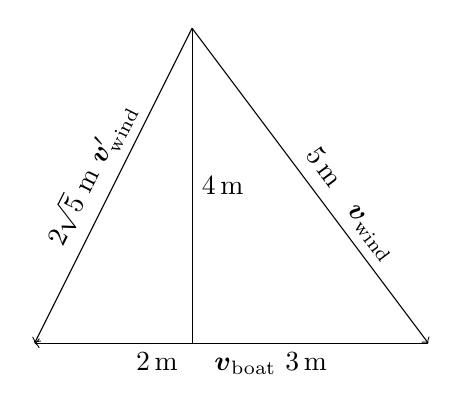
\begin{tikzpicture}
	\centering
	\draw[->] (3,-4) --node[pos=0.5,below]{\SI{2}{\metre} \quad$\boldsymbol{v}_\mathrm{boat}$ \SI{3}{\metre}}(-2,-4);
	\draw (0,-4) --node[right]{\SI{4}{\metre}} (0,0);
	\draw[<-] (-2,-4) --node[pos=0.5,above,sloped]{$2\sqrt{5}$ \si{\metre} $\boldsymbol{v}'_\mathrm{wind}$} (0,0) ;
	\draw[->] (0,0) --node[pos=0.6,above,sloped]{\SI{5}{\metre}\quad$ \boldsymbol{v}_\mathrm{wind}$} (3,-4) ;
\end{tikzpicture}
\end{center}
于是$ v_\mathrm{boat} = \SI{8}{\metre \per \second}$

\paragraph{1.19} 将质量为 $ m $ 的质点竖直向上抛入有阻力的介质中.设阻力与速度平方成正比, 即 $ R = m k^2 g v^2 $.如上掷时的速度为 $ v_0 $, 试证此质点又落至投掷点时的速度为\[ v_1 = \frac{ v_0 }{ \sqrt{1+k^2 {v_0}^2}} \]
\par 解:
上升,
\begin{gather*}
	m \dot{v} = -m g (1 + k^2 v^2) \Rightarrow
	\frac{v \  \mathrm{d} v}{\mathrm{d} y} = -g (1 + k^2 v^2) \\
	\int_{v_0}^{0} \frac{v \  \mathrm{d} v}{\mathrm{d} y} = \int_{0}^{h} -g \left( 1 + k^2 v^2 \right)  \  \mathrm{d} y \\
	\frac{1}{2 k^2} \ln \left( 1 + k^2 v_{0}^{2}\right) = gh
\end{gather*} 
下降,
\begin{gather*}
	\int_{0}^{v_1} \frac{v \  \mathrm{d} v}{\mathrm{d} y} = \int_{h}^{0} gh  \left( 1 - k^2 v^2 \right) \ \mathrm{d} y \\
	- \frac{1}{2k^2} \ln \left( 1 + k^2 v_{0}^2 \right) = gh \\
	\Rightarrow \left( 1 + k^{2} v_{0}^2 \right)  \left( 1 - k^2 v_{1}^{2} \right) = 1\\
	v_1 = \frac{v_0}{\sqrt{1+ k^2 v_0^2}}
\end{gather*}

\paragraph{1.27} 一质点自一水平放置的光滑固定圆柱面凸面的最高点自由滑下.问滑至何处,此质点将离开圆柱面?假定圆柱体的半径为 $ r $.
\par 解:设质点和中心的连线与垂直方向夹 $\theta$ 角时离开圆柱面
\begin{gather*}
	v = \sqrt{2 g r \left( 1 - \cos \theta \right) } \\
	m \frac{v^2}{r} = m g \cos \theta \\
	\Rightarrow 3 \cos \theta = 2 \\
	\theta = \arccos \frac{2}{3}
\end{gather*}
\paragraph{1.33} 光滑钢丝圆圈的半径为 $ r $, 其平面为竖直的. 圆圈上套一小环,其重为 $ W $. 如钢丝圈以匀加速度 $ a $,沿竖直方向运动,求小环的相对速度 $ v_r $ 及圈对小环的反作用力 $ R $.
\par 解:\\
设初始时刻小环和中心连线与垂直方向夹 $\theta_0$ 初始相对速率为 $v_0$, 相对速率为 $v_r$ 时夹角为 $\theta$.不妨假设加速度方向竖直向下(向上时取负值).
\begin{gather*}
	\frac{1}{2} m v_{r}^2 - \frac{1}{2} m v_{0}^2 = W \left( 1 - \frac{a}{g} \right) \left( \cos \theta_0 - \cos \theta \right) \\
	v_r =\sqrt{ v_0^2 + 2 \frac{W}{g} r \left( 1 - \frac{a}{g} \right)\left( 2 \cos \theta_0 - 3 \cos \theta \right) } 
\end{gather*}
\begin{equation*}
	\begin{aligned}
	R &= m \frac{v_r^2}{r} - W \left( 1 - \frac{a}{g} \right) \cos \theta  \\
	&= W \left[ \frac{v_0^2}{gr} + \left( 1 - \frac{a}{g}\right) \left( 2 \cos \theta_0 - 3 \cos \theta \right) \right] 
	\end{aligned}
\end{equation*}
$R \textgreater 0$ 表示向内.

\paragraph{1.37} 根据湯川核力理论,中子与质子之间的引力具有如下形式的势能: \[ V\left( r \right) = \frac{ k \mathrm{e}^{-ar}}{r} \quad \left( k \leq 0 \right)  \]\\
试求:\\
(1) 中子与质子间的引力表达式,并与平方反比定律相比较;\\
(2) 求质量为 $ m $ 的粒子作半径为 $ a $ 的圆运动的动量矩 $ J $ 及能量 $ E $.
\par 解:\\
(1).
\[F(r) = -\frac{\mathrm{d}}{\mathrm{d}r} V \left(  r \right)  = \frac{k  \mathrm{e}^{-ar}}{r^2} \left( 1 + ar \right) \] 
比平方反比律多两个因子.\\
(2).
\begin{gather*}
	F(a) = m \frac{v^2}{a} \Rightarrow v =\sqrt{\frac{k\mathrm{e}^{-a^2}}{ma}}\\
	J = m v a = \sqrt{m a k \mathrm{e}^{-a^2}} \\
	E = \frac{1}{2} m v^2 + V(a) = \frac{3k \mathrm{e}^{-a^2}}{2a}
\end{gather*}

\paragraph{1.45} 如 $ \dot{s}_a $ 及 $ \dot{s}_p $ 为质点在远日点及近日点处的速率, 试证明\[ \dot{s}_p : \dot{s}_a = (1+e) : (1-e) \]
\par 解:由角动量守恒
\[m \dot{s}_a (a+c) = m \dot{s}_p (a-c) \Rightarrow \frac{\dot{s}_p}{\dot{s}_a } = \frac{a+c}{a-c} = \frac{1+e}{1-e}\]

\end{document}
